%\VignetteIndexEntry{contextual: Simulating Contextual Multi-Armed Bandit Problems in R (article)}
%\VignetteEngine{knitr::knitr}
%\VignetteKeyword{archivsit}
%\VignetteKeyword{package}
%\VignetteKeyword{vignette}
%\VignetteKeyword{LaTeX}
\documentclass[nojss]{jss}

\usepackage[utf8]{inputenc}
\usepackage{color}

\usepackage{natbib}
\usepackage[british]{babel} % for correct word hyphenation
\raggedbottom % for blank spaces at the bottom (e.g., references section)
%\setcounter{tocdepth}{3} % for table of contents
%\setcounter{secnumdepth}{3} % setting level of numbering
%%%%%%%%%%%%%%%%%%%%%%%%%%%%%%
%% declarations for jss.cls %%%%%%%%%%%%%%%%%%%%%%%%%%%%%%%%%%%%%%%%%%
%%%%%%%%%%%%%%%%%%%%%%%%%%%%%%

%% almost as usual
\author{Robin van Emden\\JADS \And
  Eric Postma\\Tilburg University \And
  Maurits Kaptein\\Tilburg University}

\title{\pkg{contextual}: Simulating Contextual Multi-Armed Bandit Problems in R}

%% for pretty printing and a nice hypersummary also set:
\Plainauthor{Robin van Emden, Eric Postma, Maurits Kaptein} %% comma-separated
\Plaintitle{contextual: Simulating Contextual Multi-Armed Bandit Problems in R} %% without formatting
\Shorttitle{\pkg{contextual}} %% a short title (if necessary)

%% an abstract and keywords
\Abstract{A large number of statistical decision problems in the social sciences and beyond can be framed as a (contextual) multi-armed bandit problem.}

\Keywords{contextual multi-armed bandits, simulation, sequential experimentation, \proglang{R}}
\Plainkeywords{contextual multi-armed bandits, simulation, sequential experimentation, R}

%% at least one keyword must be supplied

%% publication information
%% NOTE: Typically, this can be left commented and will be filled out by the technical editor
%% \Volume{50}
%% \Issue{9}
%% \Month{June}
%% \Year{2012}
%% \Submitdate{2012-06-04}
%% \Acceptdate{2012-06-04}

%% The address of (at least) one author should be given
%% in the following format:
\Address{
  Robin van Emden\\
  Jheronimus Academy of Data Science\\
  Den Bosch, the Netherlands\\
  E-mail: \email{robin@pwy.nl} \\
  URL: \url{pavlov.tech}\\
  \linebreak
  Eric O. Postma\\
  Tilburg University\\
  Communication and Information Sciences\\
  Tilburg, the Netherlands\\
  E-mail: \email{e.o.postma@tilburguniversity.edu}\\
  \linebreak
  Maurits C. Kaptein\\
  Tilburg University\\
  Statistics and Research Methods\\
  Tilburg, the Netherlands\\
  E-mail: \email{m.c.kaptein@uvt.nl}\\
  URL: \url{www.mauritskaptein.com}\\
}

%% It is also possible to add a telephone and fax number
%% before the e-mail in the following format:
%% Telephone: +43/512/507-7103
%% Fax: +43/512/507-2851

%% for those who use Sweave please include the following line (with % symbols):
%% need no \usepackage{Sweave.sty}

%% end of declarations %%%%%%%%%%%%%%%%%%%%%%%%%%%%%%%%%%%%%%%%%%%%%%%

\begin{document}

A vignette for the \cite{contextual} paper.

%% include your article here, just as usual
%% Note that you should use the \pkg{}, \proglang{} and \code{} commands.

\section{Introduction}
%% Note: If there is markup in \(sub)section, then it has to be escape as above.

The need to make decisions permeates our lives. We are continuously making them in order to affect the world around us. Decisions range from the trivial, like ‘what should I have for breakfast?’, to the much more serious, like ‘how should a power station be controlled safely?’. Many of these decisions are now made on our behalf by automated systems. From automated stock trading systems, to cars that can navigate and drive, there are an increasing number of automated decision-making systems that already, or soon will, have an increasing effect on our lives. With the increased ubiquity of computing devices and sensors, the importance of automating decision making based on this influx of data becomes of greater interest. How should we make systems that can make these decisions for us?

The first attempts at making decision-making expert systems concentrated on the use of logic and formal reasoning. Such systems were brittle since feeding the system with sufficient ground truths is difficult and time consuming, and more importantly not all outcomes are entailed by a purely logic system especially when they are probabilistic or uncertain. More recently progress has been made towards more robust systems that take a different approach, which instead learn how to make decisions through experience. This thesis is interested in this aspect of decision-making systems, how a decision-making agent should make decisions and interact with an environment, improving their behaviour through experience. The specific decision-making problems with which we are concerned can be explained by way of examples.

--- adapt the above rigorously ---

\section{Contextual Multi-Armed Bandits}
%% Note: If there is markup in \(sub)section, then it has to be escape as above.

In the canonical multi-armed bandit (MAB) problem a gambler faces a number of slot machines, each with a potentially different payoff. It is the gamblers goal to make as much profit (or, in the case of gambling, as little loss) as possible by sequentially choosing which machine to play, learning from the observations as she goes along.

\section{Implementation of the contextual R package}
%% Note: If there is markup in \(sub)section, then it has to be escape as above.

In the canonical multi-armed bandit (MAB) problem a gambler faces a number of slot machines, each with a potentially different payoff. It is the gamblers goal to make as much profit (or, in the case of gambling, as little loss) as possible by sequentially choosing which machine to play, learning from the observations as she goes along.

\section{A basic example}
%% Note: If there is markup in \(sub)section, then it has to be escape as above.

\begin{Schunk}
\begin{Soutput}
     [,1] [,2]
[1,]  0.1  0.9
\end{Soutput}
\begin{Soutput}
[1] 0
\end{Soutput}
\end{Schunk}


\begin{figure}
\begin{center}
\begin{Schunk}
\begin{Soutput}
     [,1] [,2]
[1,]  0.1  0.9
\end{Soutput}
\begin{Soutput}
[1] 0
\end{Soutput}
\end{Schunk}
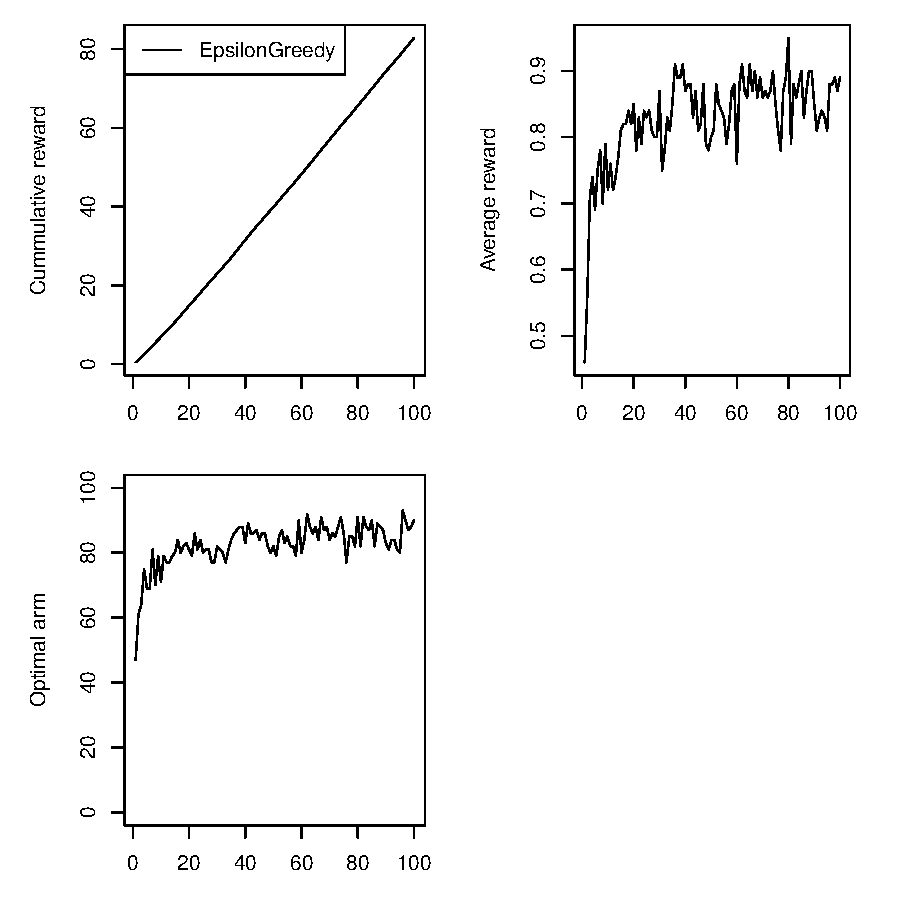
\includegraphics{jss-fig1}
\end{center}
\caption{Epsilon Greedy}
\label{fig:one}
\end{figure}


\section{Object orientation: extending contextual}
%% Note: If there is markup in \(sub)section, then it has to be escape as above.

The R6 package allows the creation of classes with reference semantics, similar to R's built-in reference classes. Compared to reference classes, R6 classes are simpler and lighter-weight, and they are not built on S4 classes so they do not require the methods package. These classes allow public and private members, and they support inheritance, even when the classes are defined in different packages.

One R6 class can inherit from another. In other words, you can have super- and sub-classes.

Subclasses can have additional methods, and they can also have methods that override the superclass methods. In this example of a custom \pkg{contextual} bandit, we’ll extend BasicBandit and override the initialize() method..

\section{Special features}
%% Note: If there is markup in \(sub)section, then it has to be escape as above.

For instance, quantifying variance..

\section{The art of optimal parallelisation}
%% Note: If there is markup in \(sub)section, then it has to be escape as above.

There is a very intersting trade of between the amount of parallelisation (how many cores, nodes used) the resources needed to compute a certain model, and the amount of data going to and fro the cores.

PERFORMANCE DATA  ------------------------------------------------------------

on 58  cores:    k3*d3 * 5 policies * 300  * 10000 --\textgreater{} 132 seconds

on 120 cores:    k3*d3 * 5 policies * 300  * 10000 --\textgreater{} 390 seconds

---

on 58  cores:    k3*d3 * 5 policies * 3000 * 10000 --\textgreater{} 930 seconds

on 120 cores:    k3*d3 * 5 policies * 3000 * 10000 --\textgreater{} 691 seconds



\section{Extra greedy UCB}
%% Note: If there is markup in \(sub)section, then it has to be escape as above.

In the canonical multi-armed bandit (MAB) problem a gambler faces a number of slot machines, each with a potentially different payoff. It is the gamblers goal to make as much profit (or, in the case of gambling, as little loss) as possible by sequentially choosing which machine to play, learning from the observations as she goes along.


\section{Conclusions}
\label{sec:conc4}

The goal of a data analysis is not only to answer a research question based on data but also to collect findings that support that answer. These findings usually take the form of a~table, plot or regression/classification model and are usually presented in articles or reports.

\section{Acknowledgments}

Thanks go to CCC.

%\bibliographystyle{apacite}
\bibliography{jss}

\end{document}
